
\chapter{A historical overview}
\label{chap:history}

\section{The theory before Gauss}

A quadratic form is a homogeneous polynomial of degree two (\emph{form}, in this
case, being a dated term for a homogeneous polynomial). The theory of quadratic
forms has a long and rich history, with some of the earliest results dating back
to antiquity. For example, integer solutions to the equation
\[
    x^2 + y^2 = z^2,
\]
commonly referred to as Pythagorean triples (although the results likely predate
the Pythagoreans), have been known to the ancient Babylonians. A table of
fifteen triples have been preserved in a tablet that has come to be labelled as
Plimpton 322 (after its provenance) and has been dated to between the 19th and
16th centuries {\lsstylehelp{100}\sc b.c.e.} \cite{robson2002words} Euclid (fl.
300 {\lsstylehelp{100}\sc b.c.e.}), in Book X, Prop.\,29, of his
\emph{Elements}, has demonstrated a way of constructing Pythagorean triples
geometrically.\,\cite{euclid1956elements} Following Euclid, the next substantial
treatment of quadratic forms (and of classical number theory, in general) was
given by Diophantus of Alexandria in his \emph{Arithmetica}, which has served as
the prototypical number theory text for much of antiquity and the Middle Ages.
\cite{katz2009history} The result that for any pair of integers \(m\) and \(n\)
with \(m > n\), the triple
\[
    (2mn, m^2 - n^2, m^2 + n^2)
\]
is Pythagorean has been known to both Euclid and Diophantus. Nevertheless, these
results have been attested to have developed separately in the Indian and
Chinese mathematical traditions during the same period. \cite{weil1984number}


\begin{figure}
    \centering
    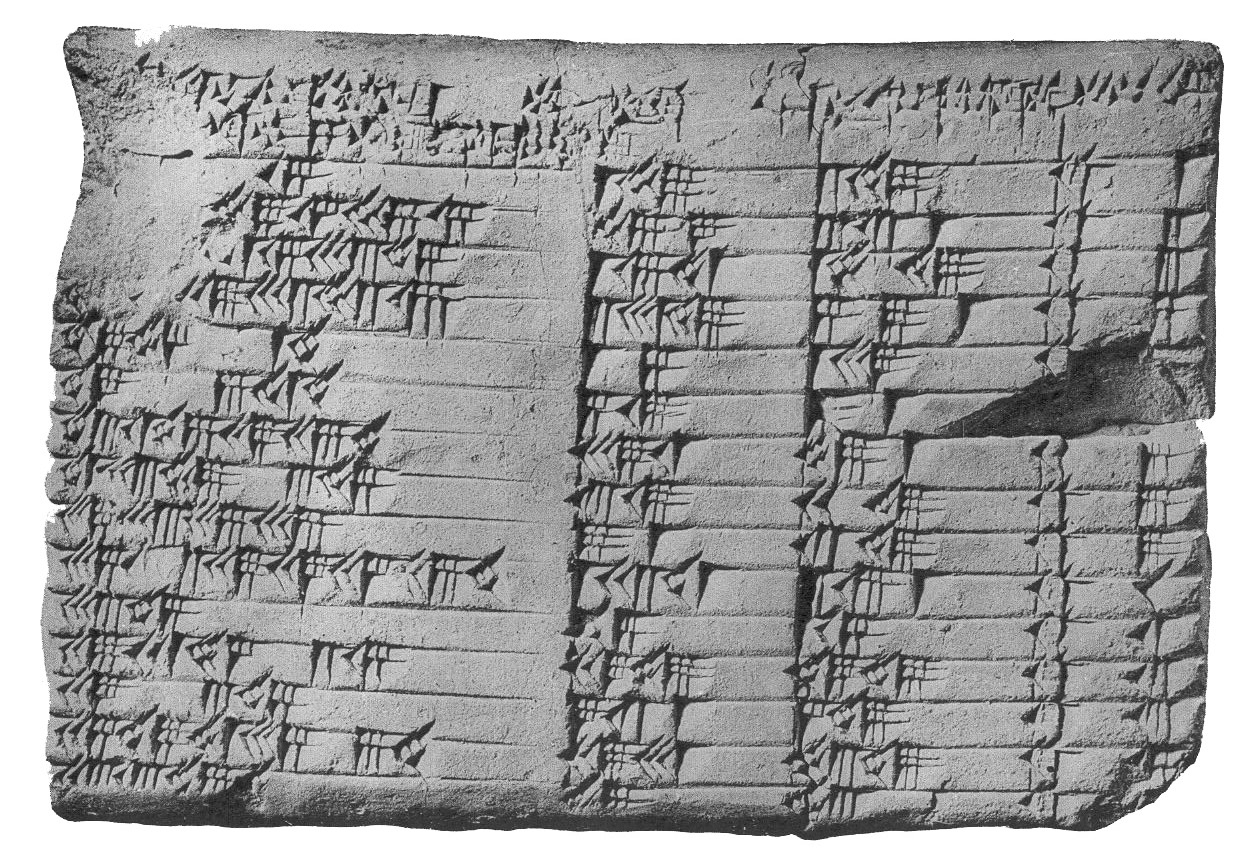
\includegraphics[width=\textwidth]{assets/Plimpton_322.jpg}
    \caption[The Plimpton 322 tablet.]{The Plimpton 322 tablet. Image from Wikimedia Commons.}
    \label{fig:plimpton-322}
\end{figure}

\begin{figure}
    \centering
    \includegraphics[width=0.8\textwidth]{assets/euclid.png}
    \caption[A geometric construction of Pythagorean triples.]{A geometric
    construction of Pythagorean triples from Euclid's \emph{Elements}. Image
    from the Greek text prepared by Heiberg. \cite{heiberg1885euclid}}
    \label{fig:pythagorean-triples}
\end{figure}


The work of Diophantus on the theory of numbers continued to be expanded upon
both by Islamic mathematicians during the Middle Ages, including in treatises by
al-Khwarizmi (fl. 800 {\lsstylehelp{100}\sc c.e.}) and European mathematicians
like Vi\`ete, Bachet, and Pacioli during the Renaissance. In the 18th century,
Pierre de Fermat and Leonhard Euler have shown that all prime numbers of the
form \(4n + 1\) can be represented by a sum of
squares.\,\cite{hahn2008quadratic} Later on Fermat and Joseph-Louis Lagrange
have expanded this to sums of the form \(x^2 + Ny^2\) for some integer \(N\).
Perhaps the most famous result of this period is Lagrange's assertion that every
whole number can be expressed as the sum of four squares. Fermat, during this
time, has introduced one of the longest-standing open problems in number theory,
his ``last theorem'' about how there are no integer solutions to the equation
\(x^n + y^n = z^n\) for \(n > 2\). While this problem is not directly related to
quadratic forms, it has significantly influenced the development of the theory
of numbers in the centuries since, culminating in a solution by Andrew Wiles in
1995. \cite{wiles1995modular}

\section{From Gauss to the fifteen theorem}

At the turn of the century, Carl Friedrich Gauss published what was to become
the most influential work on number theory, \emph{Disquisitiones Arithmetic\ae}.
It is difficult to overstate the effect that Gauss’s \emph{Disquisitiones} has
had on the development of the theory of numbers. This work is to cast a long
shadow on the work of mathematicians in the the time since its original
publication, not least because of the sheer scope of its contents. Two centuries
after \emph{Disquisitiones} first appeared, the mathematician John Conway was to
remark, for example,
\begin{quote}
    [W]hen Neil Sloane and I wanted to summarize the classification theory of
    binary forms for one of our books, we found that the only Number Theory
    textbook in the Cambridge Mathematical Library that handled every case was
    still the \emph{Disquisitiones}! \cite{conway1999universal} 
\end{quote}
In \emph{Disquisitiones}, Gauss has introduced, among other things, important
results in congruence,\,---\,a notion which remains a central concept in modern
number theory; much of the number theoretic notation still used to this day can
be traced back to this book by Gauss, in particular writing
\[
    a \equiv b \quad (\text{mod. } m)
\]
to indicate that \(a\) and \(b\) are ``congruent'' under the  ``modulus'' \(m\).
(The dot after the original abbreviation was soon to disappear.) More than half
of the six-hundred-odd pages of \emph{Disquisitiones} is devoted to the theory
of quadratic forms and quadratic reciprocity, which Gauss has exhaustively
studied. Section\,5 of the \emph{Disquisitiones} treats ``forms and
indeterminate equations of the second degree,''
\cite[Art.\,153]{gauss1801disquisitiones} --- mainly in two, and partly in
three, unknowns, --- primarily building on the previous work of Euler, Lagrange,
and Adrien-Marie Legendre.\,\cite{goldstein2007book} We also get from Gauss the
following notation for quadratic forms, which we adapt with some modifications
in this paper:
\begin{quote}
    Formam \(axx + 2bxy + cyy\), quando de indeterminatis \(x, y\) non agitur,
    ita designabimus \((a, b, c)\). \cite[Art.\,153]{gauss1801disquisitiones}

    \medskip

    \noindent\emph{The form \(axx + 2bxy + cyy\), when the indeterminates \(x,
    y\) are not in question, we shall designate by \((a, b, c)\).}
\end{quote}

Central to the theory of quadratic forms that was developed by Gauss and his
predecessors is the notion of equivalence of forms, which we state in terms of
the existence of a linear transformation that transforms one quadratic form into
another, so that one can be constructed by a linear substitution of variables
from the other. We shall formalize this notion in Chapter
\ref{chap:quadratic-forms} and establish that ``equivalence'' of forms is indeed
an equivalence relation. The notion of equivalence allows us to work not with
individual forms but with their equivalence classes, and thus attempts to
classify quadratic forms in turn become a question of classifying them up to
equivalence. Work on quadratic forms continued into the nineteenth century in
the spirit of Gauss's \emph{Disquisitiones}, primarily through the development
of various reduction theories that aim to find some unique canonical form for
each equivalence class of quadratic forms.

The reduction and classification theories in the \emph{Disquisitiones} was
completed by James Joseph Sylvester (in his famous ``law of inertia'') over the
real numbers. The French mathematician Charles Hermite has provided useful
bounds for reducing quadratic forms over \(\Integers\) using the concept of the
minimum of a positive-definite quadratic form. \cite{gerstein2008basic} (We
shall review some of these results in Chapter \ref{chap:quadratic-forms} and
again in Chapter\,\ref{chap:integral-quadratic-forms}.) Towards the end of the
nineteenth century, Hermann Minkowski introduced the ``local-global'' principle
for the classification of quadratic forms. The introduction by Kurt Hensel in
1897 of \(p\)-adic numbers, and the work on valuation theory by his student
Helmut Hasse, has allowed for the extension of the local-global principle to a
more general number-theoretic setting.
\cite{gerstein2008basic,hensel1913zahlentheorie,hasse1922uber} We shall develop
the results from Minkowski, Hensel, and Hasse as they apply to rational
quadratic forms in Chapter \,\ref{chap:local-global-principle}.

In addition to equivalence, the second fundamental notion in the theory of
quadratic forms is the of representation. Informally, we say that some value
\(\lambda\) is represented by a quadratic form if there exists some value \(x\)
such that the quadratic form evaluated at \(x\) is equal to \(\lambda\). A
significant area of mathematical interest has always been the representability
of numbers, --- and the integers, in particular, --- by quadratic forms. The
theory developed by Hesse and Hansel begin to break down when one considers
quadratic forms over not a field but a principal ideal domain like the ring
\(\Integers\) of integers.\footnote{We shall make this notion more precise
shortly, but for completeness we state that a quadratic form is defined ``over''
a field (or a ring) if its associated matrix has entries from that field (or
ring).} In the 1930s, Carl Siegel published a series of ground-breaking papers
that provided significant advances in the theory of quadratic forms over
\(\Integers\), mainly through the methods of complex analysis. Siegel explored
the gap in the applicability of the Hasse-Minkowski theorem in \(\Integers\)
using the notion of the genus of the quadratic form (an idea which traces its
roots yet again to Gauss and his \emph{Disquisitiones} and relies on the less
restrictive notion of semi-equivalence) and that of the class number, which is
the number of equivalence classes of quadratic forms in a given genus.
\cite{gerstein2008basic}

At about the same time as Siegel was developing the arithmetic theory, Ernst
Witt introduced a more geometric approach to the study of quadratic forms. We
owe to Witt the lens of understanding forms as spaces equipped with a symmetric
bilinear map and equivalence as structure-preserving mappings between these
spaces (isometries, to be more precise.) T.Y. Lam's monograph
\cite{lam1973quadratic}, on which we heavily rely in our exposition in
Chapter\,\ref{chap:quadratic-forms}, remains a comprehensive introduction to
this algebraic point of view.